\section{Implementation}\label{impl}
This section presents an overview of the implementation of SCache. 
We first present the system overview and the detail of sampling in Subsection \ref{arch}. 
The following \ref{memorymanage} subsection focuses on two constraints on memory management.
% In Subsection \ref{crossframework}, we evaluate the cross-framework capability of SCache. 
% At last, we discuss the cost of adapting SCache and fault tolerance. 
{\color{black}
In Subsection \ref{fault}, we discuss the fault tolerance of the system.
}


\subsection{System Overview}\label{arch}
{\color{black}
As shown in Figure \ref{fig:architecture}, SCache consists of three components: a distributed shuffle data management system, a DAG co-scheduler, and a worker daemon.
As a plug-in system, SCache needs to rely on a DAG framework. 
The master node of SCache includes a DAG co-scheduler and a storage manager.
The DAG co-scheduler is responsible for pre-scheduling the reduce tasks assignment and then forcing the DAG framework to assign reduce tasks according to this assignment.
The storage manager is used for managing the shuffle blocks saved in worker nodes.
% The master node of SCache coordinates the shuffle blocks globally with application context. The worker node reserves memory to store blocks.
% The coordination provides two guarantees: (a) data is stored in memory before tasks start and (b) data is scheduled on-off memory with all-or-nothing and context-aware constraints. 
% The daemon bridges the communication between DAG framework and SCache. The co-scheduler is dedicated to pre-schedule reduce tasks with DAG information and enforce the scheduling results to the original scheduler in framework.

When a DAG job is submitted, the DAG information is generated in the framework task scheduler. 
% Before the computing tasks begin, the shuffle dependencies are determined based on DAG.
% For each shuffle dependency, the shuffle ID, the type of partitioner, the number of map tasks, and the number of reduce tasks are included.
If the RangePartitioner or a customized non-hash partitioner is used, SCache will insert an extra sampling job before the job starts.
The sampling job uses a reservoir sampling algorithm \cite{reservoir} on each partition to gather the sample data.
SCache master predicts the reduce partition size based on the data and then call Algorithm \ref{hminheap} or \ref{mhminheap} to do the pre-scheduling.

% After a map task finishes computing, the shuffle write implementation of the DAG framework is modified to call the SCache API to move all the blocks out of framework worker through memory copy and release the slot immediately.
After a map task finishes computing, the shuffle writes in the map task is modified to use SCache API to memory copy all shuffle blocks to the SCache worker reserved memory.
% After that, the slot will be released (without being blocked on disk operations).
The SCache records the block ID and the size and sends them to the master.
% When a block of the map output is received, the SCache worker will send the block ID and the size to the master.
% If the collected map output data reach the observation threshold, the DAG co-scheduler will run the scheduling Algorithm \ref{hminheap} or \ref{mhminheap} to pre-schedule the reduce tasks and then broadcast the scheduling result to start pre-fetching on each worker.
If the collected shuffle blocks reach a threshold, the SCache co-scheduler will run the scheduling Algorithm \ref{hminheap} or \ref{mhminheap} to pre-schedule the reduce tasks.
After pre-scheduling, SCache workers start pre-fetching shuffle blocks according to the assignment from the master.
To enforce the DAG framework to assign tasks according to the SCache pre-scheduled results, we also insert some lines of codes in the framework scheduler.
}
% After modification, the DAG scheduler consults SCache co-scheduler to get the preferred location for each task.

% \subsubsection{Reservoir Sampling}\label{sampling}
% {\color{black}
% If the submitted shuffle dependencies contained a RangePartitioner or a customized non-hash partitioner, the SCache master will send a sampling request to the framework master. 
% The sampling job uses a reservoir sampling algorithm \cite{reservoir} on each partition. 
% % For the sample number, it can be tuned to balance the overhead and accuracy. 
% % The sampling job randomly selects some items and performs a local shuffle with the partitioner. 
% % At the same time, the items number is counted as the weight. 
% % These sampling data will be aggregated by reduce task ID on SCache master to predict the reduce partition size. 
% The result will be aggregated on SCache master to predict the reduce partition size.
% After the prediction, SCache master will call Algorithm \ref{hminheap} or \ref{mhminheap} to do the pre-scheduling.
% }

\begin{figure}
	\centering
	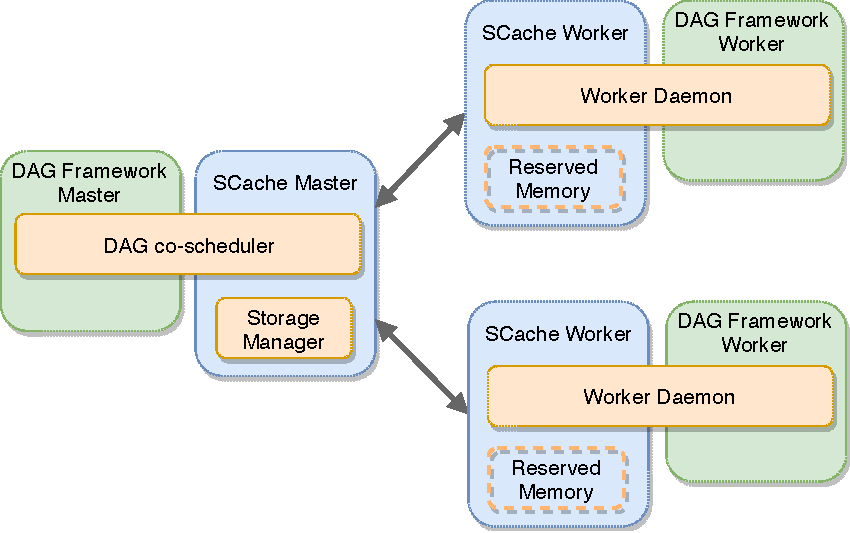
\includegraphics[width=.7\linewidth]{fig/architecture}
	\caption{\color{black}SCache Architecture}
	\label{fig:architecture}
\end{figure}

\subsection{Memory Management}\label{memorymanage}
% As mentioned in Section \ref{observation}, though the shuffle size is relatively small, memory management should still be cautious enough to limit the effect of performance of DAG framework.
{\color{black}
SCache uses bellowed memory management to ensure performance.
If the reserved memory is running out, SCache will flush some of the blocks into the disk temporarily and then re-fetch them if needed.
SCache leverages two constraints to manage the shuffle blocks: \textit{all-or-nothing} and \textit{context-aware-priority}.
% When the size of cached blocks reaches the limit of reserved memory, SCache flushes some of them to the disk temporarily, and re-fetches them when some cached shuffle blocks are consumed or pre-fetched. 
% To achieve the maximum overall improvement, SCache leverages two constraints to manage the in-memory data --- \textit{all-or-nothing} and \textit{context-aware-priority}.
}

\subsubsection{All-or-Nothing Constraint}
% This acceleration of in-memory cache of a single task is necessary but insufficient for a shorter stage completion time. 
{\color{black}
% Based on the observation in Section \ref{multi}, in most cases one single stage contains multi-rounds of tasks.
% Both experience and DAG framework manuals (e.g., Hadoop and Spark) recommend that multi-round execution of each stage will benefit the performance of applications.
As discussed in the observation in Subsection \ref{observation}, it is common to have multi-round execution of each stage. 
If one of the tasks in a round missed a memory cache, the re-fetch overhead will become a bottleneck and then slow down the whole stage. 
% If one task missed a memory cache and exceeded the original bottleneck of this round, that task might become the new bottleneck and then slow down the whole stage. 
% PACMan \cite{pacman} has also proved that for multi-round stage/job, the completion time improves in steps when $n\times number\ of\ tasks\ in\ one\ round$ of tasks have data cached simultaneously. 
% Therefore, the cached shuffle blocks need to match the demand of all tasks in one running round at least.
}
Therefore, SCache master sets blocks of one round as the minimum unit of storage management.
We refer to this as the all-or-nothing constraint.
% According to all-or-nothing constraint, SCache master leverages the pre-scheduled results to determine the bound of each round, and sets blocks of one round as the minimum unit of storage management.
% For those incomplete units, SCache marks them as the lowest priority.

\subsubsection{Context-Aware-Priority Constraint}
% Unlike the traditional cache replacement schemes such as MIN \cite{min}, the cached shuffle data will only be used once, but the legacy cache managements are designed to improve the hit rate.
{\color{black}
SCache leverages application context to select victim storage units when the reserved memory is full.
At first, SCache flushes blocks of the incomplete units to disk cluster-widely.
If all the units are completed, SCache selects victims based on two factors: 
(a) For the tasks in the different stages, SCache sets the higher priority to storage units with an earlier submission time;
(b) For the tasks in the same stage, SCache sets the higher priority to storage units with a smaller task ID.
}
% If all the units are completed, SCache selects victims based on two factors --- \textit{inter-shuffle} and \textit{intra-shuffle}.
% \begin{itemize}[noitemsep]
% 	\item Inter-shuffle: SCache master follows the scheduling scheme of Spark to determine the inter-shuffle priority. 
% 	% For example, Spark FIFO scheduler schedules the tasks of different stages according to the submission order. 
% 	SCache sets the priorities of tasks according to the submission time of each shuffle.
% 	% For a FAIR scheduler, Spark balances the resource among task sets, which leads to a higher priority for those having more tasks unfinished. 
% 	% So SCache sets priorities from high to low in a descending order of remaining storage units of a shuffle. 
% 	% For a FIFO scheduler, Spark schedules the task set that is submitted first. 
% 	% So SCache sets the priorities according to the submit time of each shuffle unit.
% 	\item Intra-shuffle: The intra-shuffle priorities are determined according to the task scheduling inside a stage.
% 	For example Spark schedules tasks with smaller ID at first. 
% 	Based on this, SCache can assign the lower priority to storage units with a larger task ID.
% \end{itemize}

% {\color{red}
% \subsection{Cost of adapting DAG frameworks}
% SCache provides API through RPC, such as \textit{putBlock(blockId)}, \textit{getBlock(blockId)}, and \textit{getScheduleResult(shuffleId)}. The concise design makes it easy to adapt DAG frameworks to enable SCache optimization. For example, it only takes about 500 lines of code in Spark to integrate SCache. By a glance of Hadoop source code, we believe that the costs of enabling SCache on MapReduce \cite{hadoop} and YARN \cite{yarn} based DAG computing framework, such as Tez \cite{tez}, are also very low.
% }

% {\color{black}
% \subsection{Analysis of cross-framework capability}\label{crossframework}
% Shuffle optimization of SCache inevitably requires the modification on the DAG frameworks. SCache provides APIs through RPC, such as \textit{putBlock (blockId)}, \textit{getBlock (blockId)}, and \textit{getScheduleResult (shuffleId)}. In order to use SCache, we mainly need to modify two parts of the frameworks: (a) The DAG scheduler should provide the DAG information and follow the pre-scheduled result of SCache; (b) The shuffle data should be transferred to SCache Storage Management.

% To prove the cross-framework capability of SCache, we adapt SCache on Hadoop MapReduce and Spark respectively. In Hadoop MapReduce, we modify codes in ResourceManager, MapTask, and ReduceTask to call SCache APIs through RPC. It takes about 380 lines of code. In Spark, we mainly modify DAGScheduler and the corresponding data fetcher. 
% It only takes about 500 lines of code. Such hundreds of lines of code modification are very small compared to the hundreds of thousands of lines of code in DAG framework. We believe that the costs of enabling SCache on other DAG computing frameworks, such as Tez, are also low.
% }

{\color{black}
\subsection{Discussion of Fault Tolerance}\label{fault}
% how to handle faults? -> maybe replication -> tradeoff
For now, SCache only restarts failed workers without recovering their data.
SCache leaves the fault handling to the DAG frameworks.
If a failure happens in a SCache worker during shuffle phases, the $getBlock$ API will return a data not found error which causes the DAG framework restarts the current stage.
During the re-computing, the DAG frameworks still use SCache to gain shuffle optimization.
A possible way to avoid this re-computing is to use replications to recover the data.
However, such replications can introduce a significant network overhead.
We believe that the current way is more promising because most DAG frameworks have more advanced fast recovery schemes on the application layer, such as the paralleled recovery of Spark. 
% Meanwhile, SCache can still provide shuffle optimization during the re-computing.
}

% Due to the characteristic of shuffle data (e.g., short-lived, write-once, read-once), we believe fault tolerance is not a crucial goal of SCache at present.
% We plan to implement SCache master with Apache ZooKeeper \footnote{https://zookeeper.apache.org/} to provide constantly service. 
% If a failure happens inside the SCache worker, SCache daemon can block the shuffle write/read operations until the worker process restarts without violating the correctness of the DAG computing.
% A possible way to handle this failure is selecting some backup nodes to store replications. 
% % But the replications can introduce a significant network overhead \cite{availability}.  
% Currently, we leave the sever faults (e.g., the failure of a node) to the DAG frameworks. 
% We believe it is a more promising way because most DAG frameworks have more advanced fast recovery schemes on the application layer, such as paralleled recovery of Spark. 
% Meanwhile, SCache can still provide shuffle optimization during the recovery.